\chapter{Réduction des endomorphismes}
\labch{reduction_des_endomorphismes}

{\Large Diagonalisation} \\
\marginnote[0cm]{Le texte suivant est extrait de \cite{oraux_x_ens_2} p. 169.}
\begin{marginfigure}[1cm]
    \centering
    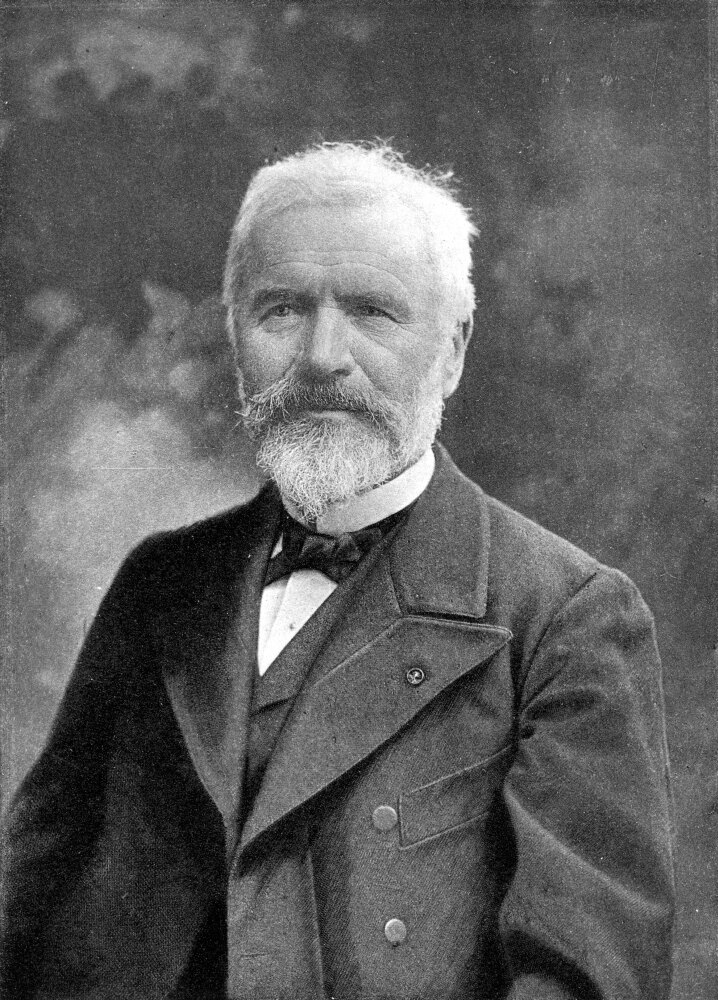
\includegraphics[width=5cm]{images/camille_jordan.jpg}
    \caption*{\centering Camille \textsc{Jordan} (1838 - 1922)}
\end{marginfigure}
\textsl{On doit à Camille \textsc{Jordan} de nombreux résultats sur la réduction des endomorphismes qu'il découvre notamment à travers l'étude des groupes. Dépassant la notion des groupes de permutations pour en atteindre une plus abstraite, il s'intéresse à la classification des groupes finis à travers leurs représentations linéaires, autrement dit les morphismes entre un groupe fini $G$ et le groupe linéaire $\Gl (E)$ d'un espace vectoriel $E$. Il va même jusqu'à donner le description des classes de similitudes à l'aide des formes dites de \textsc{Jordan}. \\
Le problème fondamental de la réduction est bien celui de caractériser les classes de similitude de l'algèbre $\Endo(E)$ où $E$ est un $\K$-espace vectoriel de dimension finie ou, ce qui revient au même, les classes de similitudes de l'agèbre $\M_n(\K)$. La recherche d'une matrice la plus simple possible pour représenter un endomorphisme donné vise de multiples buts: calculer les puissances successives de cet endomorphisme, son commutant, résoudre des systèmes différentiels linéaires... Une idée naturelle pour essayer de \say{ réduire } l'étude d'un endomorphisme $u$ donné à des choses plus simples consiste à essayer de décomposer l'espace vectoriel $E$ en une somme directe de sous-espaces non triviaux stables par $u$. Cela n'est évidemment pas toujours possible. Les sous-espaces stables les plus simples sont ceux sur lesquels $u$ coïncide avec une homothétie. On est ainsi naturellement amené à la notion de valeur propre. Si $\lambda$ est un scalaire, on s'intéresse donc au sous-espace $E_\lambda = \Ker(u - \lambda \Id_E)$ appelé sous-espace propre pour la valeur propre $\lambda$ lorsque celui-ci n'est pas nul. Le théorème de décomposition des noyaux nous assure que les différents sous-espaces propres d'un endomorphisme sont en somme directe. Le cas où la somme remplit tout l'espace $E$ mène à la notion d'endomorphisme diagonalisable: un tel endomorphisme peut être représenté par une matrice diagonale (il suffit de prendre une base formée de vecteurs propres). Pour les endomorphismes diagonalisables il est alors très facile de répondre à la question initiale de savoir quand ils sont semblables: il faut et suffit qu'ils aient les mêmes valeurs propres et que les espaces propres associés aient la même dimension. Il est aussi facile, en se ramenant à une matrice diagonale, de calculer les puissances d'un tel endomorphisme, son exponentielle (si on travaille sur un sous-corps de $\C$), son commutant...} \\

Soit $E$ un espace vectoriel de dimension finie. Un endomorphisme $u$ de $E$ est trigonalisable si et seulement s'il existe un drapeau total de $E$ stable par $u$. 

\begin{Large}
    Trigonalisation
\end{Large}

\textsl{La diagonalisation ne permet pas de caractériser toutes les classes de similitude de $\M_n(\K)$. Lorsque le corps de base est égal à $\C$, le polynôme caractéristique d'une matrice $A \in \M_n(\C)$ est toujours scindé et $A$ est alors trigonalisable. Le lemme des noyaux permet même dans ce cas de trigonaliser $A$ sous une forme diagonale par blocs avec pour chaque bloc diagonal une unique valeur propre. Cela conduit à la notion de sous-espace caractéristique et à la décomposition de \textsc{Jordan}-\textsc{Dunford}: dans le cas abstrait, tout endomorphisme $u$ d'un $\C$-espace vectoriel de dimension finie s'écrit de manière unique sous la forme $u = d + n$ où $d$ est diagonalisable, $n$ est nilpotent et commute avec $d$. (H.P. CPGE). Cette décomposition amène l'attention sur les classes de similitude des endomorphismes nilpotents. Avec un peu de travail il est alors possible d'obtenir le théorème de \textsc{Jordan} qui règle complètement la question de la détermination des classes de similitude sur un corps algébriquement clos. \\
Dans le cadre général, l'outil fondamental pour élucider les classes de similitude de $\M_n(\K)$ est la notion d'endomorphisme cyclique.
}

\newpage

\section{Matrices à diagonale dominante}
\begin{defi}
    Soit $A = (a_{i,j}) \in \M_n(\K)$. On dit que $A$ est 
    \begin{itemize}
        \item à \emph{diagonale dominante} si
        $$\forall i \in \llbracket 1, n \rrbracket,\ |a_{i,i}| \geqslant \sum_{k \not = i} |a_{i,k}|,$$
        \item à \emph{diagonale fortement dominante} si de plus l'inégalité est stricte pour une valeur de $i$ au moins,
        \item à \emph{diagonale strictement dominante} si l'inégalité est stricte pour tout $i$. 
    \end{itemize}
\end{defi}

\begin{lemme} \label{lemme_hadamard}
    Toute matrice à diagonale strictement dominante (DSD) est inversible.
\end{lemme}

\marginnote[2cm]{
    \begin{methode}
    Penser à poser 
        $$\left |x_{i_0} \right | \defeq \max_{1 \leqslant i \leqslant n} |x_i|.$$
    \end{methode}
}

\begin{preuve}
    Soit $X = \Trsp{(x_1 \cdots x_n)} \in \Ker(A)$. \\
    On pose $\displaystyle \left |x_{i_0} \right| \defeq \max_{1 \leqslant i \leqslant n} |x_i|$. La ligne $i_0$ de la relation $AX = 0$ donne
    $$\sum_{j=1}^n a_{i_0,j}x_j = 0$$
    soit
    $$-a_{i_0, i_0} x_{i_0} = \sum_{j \not = i_0} a_{i_0,j} x_j$$
    d'où, d'après l'inégalité triangulaire,
    $$|a_{i_0, i_0}| |x_{i_0}| \leqslant \sum_{j \not = i_0} |a_{i_0,j}| |x_j| \leqslant |x_{i_0}| \sum_{j \not = i_0} |a_{i_0, j}|.$$
    Comme $|a_{i_0, i_0}| > \sum\limits_{j \not = i_0} |a_{i_0, j}|$ par définition de $A$, on en déduit que
    $|x_{i_0}| = 0$, autrement dit $X = 0$. Le noyau de $A$ est donc réduit au vecteur i.e. la matrice $A$ est inversible. \\
    Pour une autre démonstration voir \cite{matrices} page 51. 
\end{preuve}

\marginnote{
    On considère la matrice à coefficients complexes
    $$
    \begin{pmatrix}
        \textcolor{red}{\mi4} & 0 & 2 & \mi3 \\
        1 & \textcolor{blue}{5+\mi10} & 5 & -1 \\
        0 & 2 & \textcolor{ForestGreen}{1} & 0 \\
        1 & 2 & 0 & \textcolor{orange}{-8-\mi2}
    \end{pmatrix}.
    $$
    Ci-dessous sont représentés ses disques de \textsc{Gerschgorin} et les croix correspondent à ses valeurs propres.
}

\begin{marginfigure}
    % This file was created with tikzplotlib v0.10.1.
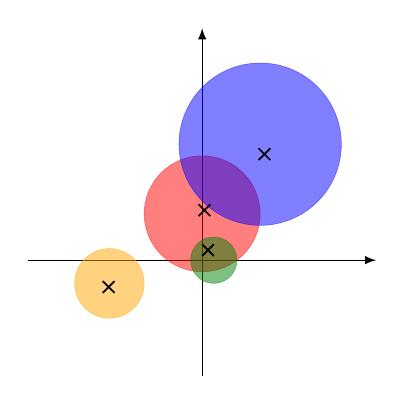
\begin{tikzpicture}

\definecolor{dimgray85}{RGB}{85,85,85}
\definecolor{gainsboro229}{RGB}{229,229,229}
\definecolor{green}{RGB}{0,128,0}
\definecolor{lightgray204}{RGB}{204,204,204}
\definecolor{orange}{RGB}{255,165,0}

\begin{axis}[
axis lines=middle,
inner axis line style={-latex},
grid=major,
width=6cm,
height=6cm,
xtick=\empty,
xmin=-15, xmax=15,
ytick=\empty,
ymin=-10, ymax=20,
]
\draw[draw=red,fill=red,opacity=0.5,very thin] (axis cs:0,4) circle (5);
\draw[draw=blue,fill=blue,opacity=0.5,very thin] (axis cs:5,10) circle (7);
\draw[draw=green,fill=green,opacity=0.5,very thin] (axis cs:1,0) circle (2);
\draw[draw=orange,fill=orange,opacity=0.5,very thin] (axis cs:-8,-2) circle (3);

\def\r{3}

%\addplot [semithick, red, mark=*, mark size=\r, mark options={solid}, only marks]
%table {%
%0 4
%};
%\addlegendentry{1\mi}
%\addplot [semithick, blue, mark=*, mark size=\r, mark options={solid}, only marks]
%table {%
%5 10
%};
%\addlegendentry{(5+10\mi)}
%\addplot [semithick, green, mark=*, mark size=\r, mark options={solid}, only marks]
%table {%
%1 0
%};
%\addlegendentry{(1)}
%\addplot [semithick, orange, mark=*, mark size=\r, mark options={solid}, only marks]
%table {%
%-8 -2
%};
%\addlegendentry{(-8-2j)}

\addplot [semithick, black, mark=x, mark size=\r, mark options={solid}, only marks, forget plot]
table {%
-8.06720901070025 -2.31297809243462
};
\addplot [semithick, black, mark=x, mark size=\r, mark options={solid}, only marks, forget plot]
table {%
5.36805383956579 9.13980083948909
};
\addplot [semithick, black, mark=x, mark size=\r, mark options={solid}, only marks, forget plot]
table {%
0.195375871819944 4.3072164295875
};
\addplot [semithick, black, mark=x, mark size=\r, mark options={solid}, only marks, forget plot]
table {%
0.503779299314509 0.865960823358021
};
\end{axis}

\end{tikzpicture}
\end{marginfigure}

\begin{theo}
    Soit $A \in \M_n(\K)$. Alors, $$\Sp(A) \subset \bigcup\limits_{i=1}^{n} \overline{\mathscr{B}} \Bigg( a_{i,i}, \sum\limits_{k \not = i} |a_{i,k}| \Bigg).$$ \\
    Ces disques sont nommés les \href{https://fr.wikipedia.org/wiki/Théorème_de_Gerschgorin}{disques de \textsc{Gerschgorin}} (cf. thème \textit{Localisation des valeurs propres}, Ch. 11 \cite{acamanes}).
\end{theo}

\begin{preuve}
    Soit $\lambda \in \Sp(A)$. La matrice $A - \lambda \I_n$ n'est pas inversible donc n'est pas à DSD i.e. pour tout $i \in \llbracket 1, n \rrbracket$,
    $$|a_{i,i} - \lambda| \leqslant \sum_{k \not= i} |a_{i,k}|.$$
    Le spectre de la matrice $A$ est donc inclus dans la réunion des disques de centre $a_{i,i}$ et de rayon $\sum\limits_{k \not=i} a_{i,k}$.
\end{preuve}    

\begin{corol}
    Soit $A \defeq (a_{i,j})_{1 \leqslant i, j \leqslant n} \in \M_n(\K)$. On note
    \begin{equation*}
        E &\defeq \bigcup\limits_{i=1}^{n} \overline{\mathscr{B}} \Bigg( a_{i,i}, \sum\limits_{k \not = i} |a_{i,k}| \Bigg) \quad
        E' &\defeq \bigcup\limits_{i=1}^{n} \overline{\mathscr{B}} \Bigg( a_{i,i}, \sum\limits_{j \not = i} |a_{j, i}| \Bigg).
    \end{equation*}
    Alors,
    $$\Sp(A) \subset E \cap E'.$$
\end{corol}

\begin{preuve}
    D'après le théorème 4.1 (lien), 
    $$\Sp(A) \subset E \text{ et } \Sp(\Trsp{A}) \subset E'.$$
    Or $\Sp(A) = \Sp(\Trsp{A})$ donc $\Sp(A) \subset E \cap E'$.
\end{preuve}    

Ce corollaire permet de restreindre davantage le domaine où se trouvent les valeurs propres d'une matrice. 

\begin{prop}
    Soit $A \in \M_n(\R)$ à DSD telle que $a_{i,i} > 0$ pour tout $i \in \llbracket 1, n \rrbracket$. Alors $\mathrm{det}(A) > 0$. 
\end{prop}

\begin{preuve}
        $\det(A) = \prod\limits_{\lambda \in \Sp(A)} \lambda$. Distinguer les vap complexes et réelles...
\end{preuve}


\section{Matrices stochastiques}
\marginnote[3cm]{
    $$
    \begin{pmatrix}
    1/2 & 1/2 & 0 \\
    3/4 & 1/8 & 1/8 \\
    0 & 1/3 & 2/3
    \end{pmatrix}
    $$
}

\begin{marginfigure}[5cm]
    \centering
    \resizebox{6.5cm}{6.5cm}{%
    \begin{tikzpicture}
        \node[state] (s1) {1};
        \node[state, below right of=s1] (s2) {2};
        \node[state, below left of=s1] (s3) {3};
    
        \draw (s1) edge[loop above] node {$1/2$} (s1);
        \draw (s1) edge[bend left] node {$1/2$} (s2);
        %\draw (s1) edge[bend right, above left] node {0} (s3);
    
        \draw (s2) edge[bend left, above right] node {$3/4$} (s1);
        \draw (s2) edge[loop right] node {$1/8$} (s2);
        \draw (s2) edge[bend right] node {$1/8$} (s3);
    
        %\draw (s3) edge[bend right] node {0} (s1);
        \draw (s3) edge[bend right] node {$1/3$} (s2);
        \draw (s3) edge[loop left] node {$2/3$} (s3);
    \end{tikzpicture}    
}

  %  \begin{tikzpicture}
  %      \node[state] (s1) {État 1};
  %      \node[state, below right of=s1] (s2) {État 2};
   %     \node[state, below left of=s1] (s3) {État 3};
 %  
 %       \draw (s1) edge[loop above] node {$p_{1,1}$} (s1);
%        \draw (s1) edge[bend left] node {$p_{1,2}$} (s2);
%        \draw (s1) edge[bend right, above left] node {$p_{1,3}$} (s3);
    
 %       \draw (s2) edge[bend left, above right] node {$p_{2,1}$} (s1);
%        \draw (s2) edge[loop right] node {$p_{2,2}$} (s2);
%        \draw (s2) edge[bend right] node {$p_{2,3}$} (s3);
    
%        \draw (s3) edge[bend right] node {$p_{3,1}$} (s1);
%        \draw (s3) edge[bend right] node {$p_{3,2}$} (s2);
%        \draw (s3) edge[loop left] node {$p_{3,3}$} (s3);
%    \end{tikzpicture}    
    \caption*{\centering Une chaîne de \textsc{Markov} et sa matrice de transition.}
\end{marginfigure}

Texte de \cite{oraux_x_ens_2} p. 59 \\
Les matrices stochastiques interviennent en probibilités. Si $X$ et $Y$ sont deux variables aléatoires à valeurs dans $E \defeq \llbracket 1, k \rrbracket$, alors la matrice $A \defeq (a_{i,j}) \in \M_k(\R)$ définie par $a_{i,j} = \P(Y = j | X = i)$ est stochastique, ce qui par définition signifie qu'on a $a_{i,j} \geqslant 0\ (1 \leqslant i, j \leqslant k)$ et $\sum\limits_{j=1}^k a_{i,j} = 1\ (1 \leqslant i \leqslant k)$. \\
L'évolution d'un système susceptible de prendre un nombre fini d'états notés $1, \dots, k$ est représentée mathématiquement par une suite $(X_n)_{n \geqslant 0}$ de variables aléatoires à valeurs dans $E$. C'est ce qu'on appelle un processus aléatoire (ou stochastique). Si $X_{n+1}$ s'obtient à partir de la valeur de $X_n$ et d'un tirage au sort effectué selon une loi ne dépendant que de cette valeur, on dit que le processus est une chaîne de \textsc{Markov}. Les exemples abondent: marches aléatoires, fortune d'un joueur, modélisation de l'alternance des voyelles et des consonnes dans un poème de \textsc{Pouchkine} (par \textsc{Markov} lui-même), ou prévision (en probabilité) des états  successifs d'un signal pour améliorer la compression en traitement du signal (\textsc{Shannon}) \\
Techniquement, on dit qu'une suite de variables aléatoires $(X_n)$ est une chaîne de \textsc{Markov} si \say{ la loi de l'état $n+1$ conditionnelle au passé de dépend que de l'état antérieur $n$ }, ce qui se traduit par
$$\P(X_{n+1}=j | X_0=i_0, \dots, X_n = i_n) = \P(X_{n+1} = j | X_n = i_n).$$
Si la matrice $(A) \defeq (a_{i,j}) \in \M_k(\R)$ définie par $a_{i,j} = \P(X_{n+1} = j | X_n = i)$ est indépendante de $n$, on dit que la chaîne de \textsc{Markov} est stationnaire. Si, dans ce dernier cas, on pose $Y_n \defeq \begin{pmatrix} \P(X_n = 1) \\ \vdots \\ \P(X_n = k) \end{pmatrix}$, pour tout $n \geqslant 0$, on obtient $Y_{n+1} = A Y_n$ et donc $Y_n = A^n Y_0$. \\
Le comportement (probabiliste) d'une chaîne de \textsc{Markov} stationnaire, et notamment son comportement asymptotique, est donc entièrement décrit par la donnée de la loi initiale $Y_0$ et des puissances de la matrice $A$. 

\begin{defi}
    Une matrice stochastique (matrice de transition d'une \nameref{chaîne_markov}) est une matrice $P \in \M_n([0, 1])$ telle que pour tout $i \in \llbracket 1, n \rrbracket, \sum\limits_{j=1}^{n} p_{i,j} = 1$. \\ Autrement dit, chaque ligne de $P$ est une vecteur de probabilité. \\
    On dit que $P$ est \emph{doublement stochastique} si $P$ et $\Trsp{P}$ sont stochastiques.
\end{defi}

\begin{exercice}
    \footnote{Exercice 5, TD 11} \\
    Soit $P$ une matrice stochastique.
    \begin{enumerate}
        \item Montrer que $1$ est valeur propre de $P$.
        \item Soit $v = \Trsp{(v_1 \cdots v_n)}$ un vecteur propre associé à la valeur propre $1$. En considérant $|v_{i_0}| = \max\limits_{1 \leqslant i \leqslant n} |v_i|$, montrer que le sous-espace propre associé à $E_1$ est de dimension $1$.
        \item Montrer que si $\lambda \in \C$ est une valeur propre de $P$, alors $| \lambda | \leqslant 1$.
        \item Soit $\lambda \in \C$ une valeur propre de $P$ telle que $|\lambda| = 1$ et $\title{x}$ un vecteur propre associé.
        \begin{enumerate}
            \item Montrer qu'il existe un vecteur propre associé à $\lambda$ tel que $\Ninf{x} = 1$. 
            \item Montrer qu'il existe $i_0 \in \llbracket 1, n \rrbracket$ tel que $\left| \sum\limits_{j=1}^n p_{i_0,j} x_j \right| = 1$.
            \item Soit $\theta$ l'argument principal de $\sum\limits_{j=1}^n p_{i_0,j} x_j$. Montrer que pour tout $j \in \llbracket 1, n \rrbracket, \Reel \left( \me^{-\mi \theta} x_j \right) = 1$.
            \item En déduire que $\lambda = 1$.
        \end{enumerate}
    \end{enumerate}
\end{exercice}

\begin{solution}
    L'objectif de l'exercice est de montrer que $\boxed{\Sp_{\C}(P) = \{1 \} }$.
    \begin{enumerate}
        \item 1 est valeur propre évidente de $P$ de vecteur propre associé $v = (1, \dots, 1)^\top$.
        \item Montrer que $\dim E_1 = 1$.
        \begin{itemize}
            \item Appliquer la même méthode que la démonstration du lemme d'\textsc{Hadamard}. \\
            Soit $X = \Trsp{(x_1, \dots, x_n)} \in E_1$. Montrons que $X \in \Vect(v)$. \\
            On montre que $|x_{i_0}| = \left| \sum\limits_{j=1}^{n} p_{i_0, j} x_j \right| = \sum\limits_{j=1}^{n} p_{i_0, j} |x_j|$ et on écrit $|x_{i_0}| = |x_{i_0}| \sum\limits_{j=1}^{n} p_{i_0, j}$. D'où, en faisant la différence, pour tout $j \in \llbracket 1, n \rrbracket,\ |x_{i_0}| = |x_j|$. De plus d'après la première relation, il y égalité dans l'inégalité triangulaire et donc les $v_j$ sont \emph{positivement liées}. Finalement, pour tout $j \in \llbracket1, n \rrbracket,\ v_j = v_{i_0}$ soit $\dim E_1 = 1$.
        \end{itemize}
        \item Montrer que si $\lambda \in \C$ est une valeur propre de $P$, alors $|\lambda| \leqslant 1$. \\
        Poser $X = (x_1, \dots, x_n)^\top$ un vecteur propre associé et appliquer encore une fois la même méthode; poser $\displaystyle |x_{i_0}|= \max_{1 \leqslant i \leqslant n} |x_i|$, écrire en module la ligne $i_0$ de l'égalité $\lambda X = P X$, diviser par $|x_{i_0}|$ (qui est non nul d'après la question précédente) puis majorer par $1$. \\
            
        Pour les curieux, lire \cite{matrices} page 59. 
        
        \begin{prop}
            Le \nameref{rayon_spectral} stochastique est égal à $1$.
        \end{prop}
    
        \item Les questions suivantes (à détailler éventuellement) consiste encore au même jeu avec la ligne $i_0$ et les propriétés de matrices stochastiques. 
    \end{enumerate}
\end{solution}


\section{Condition nécessaire et suffisante de diagonalisabilité dans \texorpdfstring{$\C$}{C}}
\begin{exercice} \footnote{Exercice 10 TD 11} \\
    Soit $f \in \mathscr{L}(\K^n)$.
    \begin{enumerate}
        \item On suppose que $f$ est diagonalisable. Montrer que tout sous-espace de $\K^n$ stable par $f$ admet un supplémentaire stable par $f$.
        \item Que dire de la réciproque dans $\C$.
        \item Décrire un contre-exemple à la réciproque dans $\R$, en dimension 2.
    \end{enumerate}
\end{exercice}  

\begin{enumerate}
    \item Soit $F$ un sev de $E$ stable par $f$.
    \begin{itemize}
        \item Posons $\boxed{g = f_{\vert F}}$ qui est diagonalisable car $f$ l'est par hypothèse. 
        \item Soit $\mathscr{B}_F$ une base de $F$ formée de vep de $g$. 
        \item Soit $\mathscr{B}'$ une base de $E$ formée de vep de $f$ (qui existe car $f$ est diagonalisable).
        \item On \textbf{complète} $\mathscr{B}_F$ est une base $\mathscr{B}$ de E en prenant des vep $(\varepsilon_1, \cdots, \varepsilon_r)$ de $\mathscr{B}'$. On note $(\lambda_1, \dots, \lambda_r)$ les valeurs propres associées. 
        \item On pose G = $\mathrm{Vect}(\varepsilon_1, \dots, \varepsilon_r)$. De cette manière, $F$ et $G$ sont supplémentaires. Montrons que $G$ est stable par $f$. \\
        Soit $x = \sum\limits_{i=1}^{r} \mu_i \varepsilon_i \in G$. Donc $f(x) = \sum\limits_{i=1}^{r} \mu_i f(\varepsilon_i) =  \sum\limits_{i=1}^{r} \mu_i \lambda_i \varepsilon_i \in G$ et $G$ est stable par $f$.
    \end{itemize}
    
    \item Que dire de la réciproque dans $\C$ ? \\
    Montrons que $f$ est diagonalisable. On va montrer que $E = \bigoplus\limits_{\lambda \in \Sp(f)} E_\lambda (f)$.
    
    \begin{enumerate}
        \item \underline{Somme directe:} \\
        On pose $F = \bigoplus\limits_{\lambda \in \Sp(f)} E_\lambda (f)$ et $\Sp(f) = (\lambda_1, \dots, \lambda_r)$. \\
        Soit $x = \sum\limits_{i=1}^{r} x_i \in F$ où $x_i \in E_{\lambda_i}(f)$. Alors $f(x) = \sum\limits_{i=1}^{r} \underbrace{\lambda_i x_i}_{\in E_{\lambda_i}(f)} \in F$. Donc $F$ est stable par $f$.
        \item Montrons que $F = E$. \\
        Par hypothèse, $F$ admet un supplémentaire $G$ dans $\C^n$, stable par $f$. Montrons que $\boxed{G = \{0\}}$ en raisonnant par l'absurde. \\
        On pose $\boxed{g = f_{\vert F}}$. D'après le \textbf{théorème de \textsc{D'Alembert-Gauss}} sur $\C$, $g$ admet au moins une valeur propre $\mu \in \C$ de vep associé $x_\mu$. On montre que $x_\mu \in F \cap G$. Or $F$ et $G$ sont supplémentaires donc $x_\mu = 0_E$: contradiction. D'où le résultat. 
    \end{enumerate}
    \item Décrire un contre-exemple à la réciproque dans $\R$, en dimension 2. \\
    Considérer $R_\theta$. \textcolor{green}{à revoir}
\end{enumerate}

\section{Autour du commutant}
\marginnote[0cm]{Exercice 12 TD 11}

\begin{defi}
    Soient $A \in \M_n(\R)$ et $C(A) \defeq \{ M \in \M_n(\R);\ MA = AM \}$.
\end{defi}

\emph{Toutes les questions ne sont pas abordées}

\begin{enumerate}
    \item \emph{Montrer que C(A) est un sous-espace vectoriel de $\M_n(\R)$.} \\
    Au lieu de redémontrer les propriétés d'un sev, on peut voir $C(A)$ comme le \textbf{noyau de l'application linéaire} $M \mapsto MA - AM$ ce qui donne directement le résultat. 
    \item \emph{Montrer que si $M \in C(A)$ et $M$ est inversible, alors $M^{-1} \in C(A)$.} \\
    On veut montrer que $M^{-1} A = A M^{-1}$ i.e. $A = M A M^{-1}$ ce qui est vrai car $M A = A M$.
    \item \emph{Soit $D$ une matrice diagonale dont les coefficients diagonaux notés $(d_i)_{i \in \llbracket 1, n \rrbracket}$ sont deux à deux distincts. Déterminer $C(D)$ et montrer que $\mathscr{B} = (I_n, D, \dots, D^{n-1})$ est une base de $C(D)$.}
    \begin{itemize}
        \item $C(D) = \mathscr{D}_n$ (l'ensemble des matrices diagonales de taille $n$) \textcolor{red}{(ne pas oublier de montrer la double inclusion)}.
        \item Comme $| \mathscr{B} | = \dim C(D)$, il suffit de montrer la liberté de $\mathscr{B}$. \\
        Soit $(\lambda_0, \dots, \lambda_{n-1}) \in \R^n$ tel que $\sum\limits_{k=0}^{n-1} \lambda_k D^k = 0_n$. \\
        \textcolor{green}{Revoir le caractère générateur avec les polynômes d'interpolation.}
        \begin{itemize}
            \item Pour tout $i \in \llbracket 1, n \rrbracket$, $\sum\limits_{k=0}^{n-1} \lambda_k d_i = 0_n \quad (*)$. Donc le polynôme $P = \sum\limits_{k=0}^{n-1} \lambda_k X^k$ qui est de dégré $n-1$ et prossède $n$ racines distinctes et est donc le polynôme nul. On en déduit que les $\lambda_i$ sont tous nuls. La famille $\mathscr{B}$ est bien libre et forme une base de $C(D)$.
            \item Les relations $(*)$ forment un système de \textsc{Vandermonde} de $n$ équations à $n$ inconnues. Comme les coefficients $d_i$ sont deux à deux distincts, le système est inversible et son unique solution est le vecteur colonne nul.
        \end{itemize}
    \end{itemize}
    \item On se limite au cas $n = 2$. 
    \begin{enumerate}
        \item Déterminer les matrices $A$ telles que $\dim C(A) = 4$. \\
        $C(A) = \M_2(\R)$ car $C(A) \subset \M_2(\R)$ et il y égalité des dimensions. \\
        \textbf{Évaluer les commutant en les matrices de la base canoniques de $\M_2(\R)$}: on trouve que A est scalaire. \\
        \textcolor{red}{Ne pas oublier de montrer la réciproque}. 
        \item Montrer que $\dim C(A) \geqslant 2$. \\
        Si $A$ est scalaire, cf. question précédente. \\
        Sinon montrer que la famille $\{ \I_2, A \} \subset C(A)$ est libre. 
        \item Enoncé... \\
    \end{enumerate}
\end{enumerate}

\section{Que dire si \texorpdfstring{$M^2$}{M^2} est diagonalisable ?}
\begin{prop}{Critère de diagonalisabilité}
    Soient $n \in \Ne$ et $M \in \M_n(\C)$. On suppose que la matrice $M^2$ est diagonalisable. Alors $M$ est diagonalisable si et seulement si $\Ker M = \Ker M^2$.
\end{prop}

\begin{preuve}
    \begin{itemize}
        \item[$(\Rightarrow)$] 
        %$(\Rightarrow)$ On suppose que $M$ est diagonalisable (et donc $f$ aussi). Notons $(\lambda_1, \dots, \lambda_n) \in \C^n$ les valeurs propres de $f$. Il existe une base $\mathscr{B}$ telle que $\mathrm{Mat}_{\mathscr{B}}(f) = \mathrm{Diag}(\lambda_1, \dots, \lambda_n)$. Donc $\mathrm{Mat}_{\mathscr{B}}(f^2) = \mathrm{Diag}(\lambda_1^2, \dots, \lambda_n^2)$. \\
        Supposons que la matrice $M$ est diagonalisable. Montrons que $\Ker M^2 \subset \Ker M$ (l'autre inclusion est toujours vraie) \note . \\
        \marginnote[0cm]{\note 
            Soit $X \in \Ker M$. Alors,
            $$MX = 0$$
            d'où 
            $$M (M X) = M \times 0 = 0$$
            et 
            $$X \in \Ker M^2.$$
        }
        Voyons deux approches.
        \begin{itemize}
            \item Nous allons montrer \ptnclegras{l'égalité des dimensions} de ces deux espaces. \\
            Soient $u$ l'endomorphismes canoniquement associé à $M$ et $\mathscr{B}$ une base de diagonalisation de $u$. \ptnclegras{Le rang d'une matrice diagonale étant le nombre de coefficients diagonaux non nuls}, $\Rg \Mat_\mathscr{B}(u^2) = \Rg  \Mat_\mathscr{B}(u)$ donc $\Rg u^2 = \Rg u$ \note.
            \marginnote[0cm]{\note Le rang est un invariant de similitude.}
            Par le \ptnclegras{théorème du rang}, il s'ensuit que $\dim \Ker u^2 = \dim \Ker u$.
            \item Soit $X \in \Ker M^2$ i.e. $M^2 X = 0\ (\star)$. Montrons que $MX = 0$. L'idée est de \ptnclegras{faire apparaître un produit scalaire} sur l'ensemble des vecteurs colonnes d'une matrice i.e. une produit de la forme $N^\top N$. \\
            Comme $M^2$ est diagonalisable, il existe $P$ inversible et $D$ diagonale telles que $M^2 = PDP^{-1}$. En remplaçant $M^2$ par cette expression dans $(\star)$ puis en multipliant à gauche successivement par $P^{-1}$,  $(P^{-1})^\top$ et $X^\top$ on trouve $X^\top (P^{-1})^\top D^2 P^{-1} X = 0$ soit 
            $$(D P^{-1} X)^\top (D P^{-1} X) = 0.$$
            Comme $(C, C') \mapsto C^\top \times C'$ définit un produit scalaire sur l'espace des vecteurs colonnes, on a $D P^{-1} X = 0$ car il est orthogonal à lui-même et donc, en multipliant à gauche par $P$, nous obtenons bien $MX = 0$. 
        \end{itemize}
        \item[$(\Leftarrow)$] Supposons que $\Ker M = \Ker M^2$. Voyons encore deux approches.
        \begin{itemize}
            \item \cite{reduc_des_endo} p. 100 \note 
            \marginnote[0cm]{\note La clé de cette démonstration est l'équivalence
                \begin{center}
                    $M$ diagonalisable $\Leftrightarrow$ $\exists P \in \mathrm{Ann}(M)$ \textsc{sars}.
                \end{center}
            }
            \\
            Comme $M^2$ est diagonalisable, il existe $Q$ scindé à racines simples vérifiant $Q(0) \not= 0$ tel que $X Q(X)$ annule $M^2$, c'est-à-dire $M^2 Q(M^2) = 0$. \\
            Alors, pour tout $X \in E$, $Q(M^2)X \in \Ker M^2$; or $\Ker M^2 = \Ker M$ par hypothèse donc $Q(M^2)X \in \Ker M$ soit $M Q(M^2)X = 0$. \\
            Ainsi, $XQ(X^2)$ est un polynôme annulateur de $M$. Il suffit de remarquer que ce polynôme est scindé à racines simples (car les racines complexes de $Q$ sont deux à deux distinctes et non nulles) pour conclure avec le critère algébrique de diagonalisabilité que $M$ est diagonalisable.
            \item 
            Une démonstration alternative consiste à montrer que, pour tout $\lambda \in \Ce$ de racines carrées distinctes $\mu$ et $\mu'$, le sous-espace propre $u^2$ associé à $\lambda$ se décompose avec les sous-espaces propres $u$:
            $$\Ker(\lambda \Id_E - u^2) = \Ker(\mu \Id_E - u) \oplus \Ker(\mu' \Id_E - u).$$
            La condition porte alors que le sous-espace propre de $u^2$ associé à $0$, c'est-à-dire $\Ker(u^2)$.
            \underline{Notes de cours à traiter} \\
            Raisonnons par analyse-synthèse: soit $\lambda$ une valeur propre non nulle de $f^2$. Notons $\mu$ une racine carrée complexe de $\lambda$. Montrons que $E_{\lambda}(f^2) = E_{\mu}(f) \oplus E_{-\mu}(f)$. \\
            On pose $y = \frac{x}{2} + \frac{f(x)}{2 \mu}$ et $z = \frac{x}{2} - \frac{f(x)}{2 \mu}$. \\
            Comme $f^2$ est diagonalisable, $E$ est la somme directe des sous-espaces propres de $f^2$. On décompose chacun de ces sep comme ci-dessus et on en déduit que $E$ est la somme directe des sep de $f$ i.e. $f$ est diagonalisable. \\

        \end{itemize}
    \end{itemize}
\end{preuve}


\section{Spectre de \texorpdfstring{$\Id_E-uv$ et $\Id_E-vu$}{IdE-uv et IdE - vu}} \label{spectre_I-uv_et_I-vu}
\begin{exercice}
    \marginnote[0cm]{\cite{exos_oraux}}
    Soient $u$ et $v$ deux endomorphismes d'un espace $E$ de dimension finie $n \in \Ne$. Prouver que $\Id_E - uv$ et $\Id_E - vu$ ont les mêmes valeurs propres. \\
    En déduire que $\Id_E - uv$ est inversible si $\Id_E - vu$ l'est aussi, relier les inverses.
\end{exercice}

Soient $u$ et $v$ deux endomorphismes d'un espace $E$ de dimension $n$.

\begin{enumerate}
    \item Montrer que $\Id_E-uv$ et $\Id_E-vu$ ont les mêmes valeurs propres.
    \begin{itemize}
        \item Montrer que ces deux endomorphismes ont même polynôme caractéristique en posant les deux matrices
        $$
        A = 
        \begin{pmatrix}
            U & \lambda \I_n \\
            \I_n & V
        \end{pmatrix}
        \text{ et }
        B = 
        \begin{pmatrix}
            V & -\lambda \I_n \\
            -\I_n & 0_n
        \end{pmatrix}.
        $$
        \begin{align*}
            \det(AB) &= \det(BA) \\
            (-\lambda)^n \det(AB - \lambda \I_n) &= (-\lambda)^n \det(BA - \lambda \I_n)
        \end{align*}
    \end{itemize}
    \item En déduire que $\Id_E-uv$ est inversible si et seulement si $\Id_E-vu$ l'est, relier les inverses. 
    \begin{itemize}
        \item $f \in \Gl(E) \Longleftrightarrow 0 \not \in \Sp(f)$
        \item Évaluer le résultat précédent en $\lambda = 1$.
        \item Analogie avec l'inversion par sommation géométrique des endomorphismes nilpotents (cf. \nameref{indice_nilpotence})
    \end{itemize}
\end{enumerate}

\section{Raciné carrée d'une matrice}
\url{https://share.miple.co/content/CtwFAB5leFp4M}

\begin{box_titre}{DS6}
    On note $\mathrm{Rac}(A) = \{ R \in \M_n(\R),\ R^2 = A \}$. \\
    $\blacktriangleright$ Soit $A \in \M_n(\R)$. $\mathrm{Rac}(A)$ est une partie fermée de $\M_n(\R)$. \\
    $\blacktriangleright$ $\mathrm{Rac}(\I_n)$ n'est pas une partie bornée de $\M_n(\R)$ pour $n \geqslant 3$. 
\end{box_titre}

\begin{prop}{}
    Pour tout $A \in \mathscr{S}_n^+(\R)$, il existe une unique matrice $B \in \mathscr{S}_n^+(\R)$ telle que $A = B^2$. 
\end{prop}
\textcolor{red}{retrouver la source}
\begin{preuve}
    \underline{Existence:} comme la matrice $A$ est symétrique et positive, d'après le théorème spectral, il existe $\lambda_1, \dots, \lambda_r$ des réels positifs et $P \in \mathcal{O}_n(\R)$ tels que $A = \Inv{P} \Diag(\lambda_1, \dots, \lambda_r) P$. \\
    On pose $B = \Inv{P} \Diag(\sqrt{\lambda_1}, \dots, \sqrt{\lambda_r}) P$. \\
    La matrice $B$ vérifie $B^2 = A$, elle est bien symétrique car la matrice $P$ est orthogonale et $B$ est positive puisque symétrique à valeurs propres positives. \\
    \underline{Unicité:} supposons donné une matrice $C$ comme second candidat. \\
    Considérons $Q$ un polynôme vérifiant, pour $1 \leqslant i \leqslant r, Q(\lambda_i) = \sqrt{\lambda_i}$. Ainsi, 
    $$Q(A) = \Inv{P} Q\left(\Diag(\lambda_1, \dots, \lambda_r)\right) P = \Inv{P} \Diag(\sqrt{\lambda_1}, \dots, \sqrt{\lambda_r}) P = B.$$
    Par ailleurs, comme $C^2 = A$ alors $C$ et $A$ commutent. Par conséquent, $C$ commute avec tout polynôme en $A$ et commute donc avec $B$. \\
    Les matrices $B$ et $C$ étant diagonalisables (car symétriques) et commutant, elles sont codiagonalisables. \\
    Ainsi, il existe $R \in \Gl_n(\R)$, $D_1, D_2 \in \mathscr{D}_n(\R)$ telles que $\Inv{R}BR = D_1$ et $\Inv{R}CR = D_2$. \\
    Or $D_1^2 = \Inv{R} B^2 R = \Inv{R} A R = \Inv{R} C^2 R = D_2^2$. Les matrices $D_1$ et $D_2$ étant diagonales à coefficients positifs, on en déduit que $D_1 = D_2$. Ainsi, $B = C$.
\end{preuve}

\begin{exercice}
    \underline{Exercice 11, TD 11:}\\
    Soit $A = 
    \begin{pmatrix}
        -1 & 2 & 3 \\
        0 & - 1 & 4 \\
        0 & 0 & 1
    \end{pmatrix}. 
    $ Montrer que $A$ n'a pas de racine dans $\M_3(\R)$. 
\end{exercice}


\section{Réduction d'une matrice creuse}
\begin{tcolorbox}
    Soit $n \geqslant 2$. On pose:
    $$
    A = 
        \begin{pmatrix}
              &        &   & c \\
              &  (0)   &   & \vdots \\
              &        &   & c \\
            b & \cdots & b & a
        \end{pmatrix}
        \in \M_n(\R).
    $$
    Étudier la possibilité de diagonaliser $A$ sur $\R$.
\end{tcolorbox}

\underline{Remarques:}\\
$\blacktriangleright$ Si $b = c$ alors $A$ est symétrique réelle donc diagonalisable. \\
$\blacktriangleright$ $A$ est au plus de rang 2. Donc par le \textbf{théorème du rang}, 0 est une valeur propre de $A$ de multiplicité au moins $n-2$.

\section{Vecteurs propres de \texorpdfstring{$\Trsp{\com(A)}$}{la transposée de la comatrice}}
\begin{exercice}
    Soit $A \in \M_n(\K)$ et $B = \Trsp{\com(A)}$. Montrer que les vecteurs propres de $A$ sont des vecteurs propres de $B$. 
\end{exercice}

$$\boxed{A \times\ \com(\Trsp{A}) = \com(\Trsp{A}) \times A = \det(A) \I_n}$$

\begin{elem_sol}
    Soit $\lambda \in \Sp(A)$ et $X$ un vecteur propre associé. Alors $\lambda (BX) = \det(A) X$. 
        
    \begin{itemize}
        \item $\lambda \not = 0$: $BX = \frac{\det(A)}{\lambda}X$. 
        \item $\lambda = 0$: alors $\det(A) = 0$ et $\Rg(A) \leqslant n-1$. 
        \begin{itemize}
            \item $\Rg(A) \leqslant n-2$: supposer par l'absurde qu'il existe un déterminant mineur de $A$ non nul. 
            \item $\Rg(A) = n-1$: $X \in \Ker(A)$ qui est une droite vectorielle. 
            $$\boxed{A \text{ et } B \text{ commutent donc } \Ker(A) \text{ est stable par } B}$$
        \end{itemize}
    \end{itemize}
\end{elem_sol}


\section{Éléments propres de \texorpdfstring{$MN$}{MN}, de \texorpdfstring{$NM$}{NM}}
\begin{prop}{}
    Soient $M$ et $N$ dans $\M_n(\K)$.
    \begin{itemize}
        \item $$0 \in \Sp(MN) \Longleftrightarrow 0 \in \Sp(NM)$$
        \item Soit $\lambda \in \Ke$,
        $$\dim E_\lambda(MN) = \dim E_\lambda(NM)$$
    \end{itemize}
\end{prop}

Soit $M, N \in \M_n(\K)$. 
\begin{enumerate}
    \item ...
    \item \emph{Soit $\lambda \in \Ke$, montrer que $\dim(E_\lambda (MN)) = \dim(E_\lambda (NM))$.} \\
    On remarque que si $X \in E_\lambda (MN)$ alors $NX \in E_\lambda (NM)$. On pose alors:
    \begin{alignat*}{2}
        \varphi\ :\ E_\lambda (MN)\ &\longrightarrow\ E_\lambda (NM)\\
        X\ &\longmapsto\ NX
    \end{alignat*}
    On montre que $\varphi$ est injective et on en déduit que $\dim(E_\lambda (MN)) \leqslant \dim(E_\lambda (NM))$. Par symétrie des rôles de $M$ et de $N$, on montre l'inégalité dans le sens inverse et on en déduit l'égalité.
    \item ...
    \item ...
\end{enumerate}

\begin{defi}{Partie dense}
    \marginnote[0cm]{\url{https://www.bibmath.net/dico/index.php?action=affiche&quoi=./d/dense.html}}
    Soit $E$ un espace vectoriel normé et $D$ une partie de $E$. On dit que $D$ est \emph{dense} dans $E$ si l'une des conditions équivalentes suivantes est vérifiée:
    \begin{itemize}
        \item pour tout $x \in E$, il existe une suite $(y_n)$ d'éléments de $D$ qui converge vers $x$.
        \item pour tout $x \in E$, pour tout $\varepsilon > 0$, il existe $y \in D$ tel que $\norme{y - x} \leqslant \varepsilon$.
        \item l'adhérence $\overline{D}$ de $D$ est égale à $E$.
    \end{itemize}
\end{defi}

\subsection{Densité de \texorpdfstring{$\Gl_n(\C)$}{GL_n(C)} dans \texorpdfstring{$\M_n(\C)$}{M_n(C)}}

\begin{theo}{}
    L'ensemble des matrices inversibles de $\M_n(\C)$ est dense dans $\M_n(\C)$.
\end{theo}

\begin{marginfigure}[2cm]
    \centering
    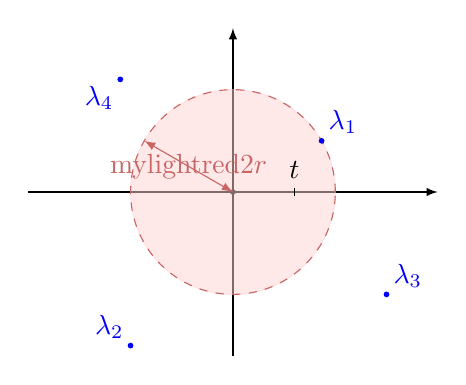
\begin{tikzpicture}[scale=1.3]
  \definecolor{mylightred}{RGB}{255,210,210}
  \definecolor{myred}{RGB}{200,100,100}
  \definecolor{mylightred2}{RGB}{255,232,232}
      \def\ang{150}
      \def\R{1}
      \coordinate (O)  at (0, 0);
      \coordinate (L1) at (30:1);
      \coordinate (L2) at (-1, -1.5);
      \coordinate (L3) at (1.5, -1);
      \coordinate (L4) at (1.2, 1);
      \coordinate (L5) at (-1.1, 1.1);
     
      \draw[-latex] (0, -1.6) -- (0, 1.6);
      \draw[-latex] (-2, 0) -- (2, 0);
      \fill[radius=0.8pt,black] (O) circle;
      \draw[mylightred, fill, opacity=0.5] (O) circle (\R);
      \draw[myred, dashed] (O) circle (\R);
      \fill[radius=0.8pt,blue]
        (L1) circle node[above right=-1pt] {$\lambda_1$}
        (L2) circle node[above left =-1pt] {$\lambda_2$}
        (L3) circle node[above right=-1pt] {$\lambda_3$}
        (L5) circle node[below left =-1pt] {$\lambda_4$};
      \draw (0.6, -0.04) -- (0.6, 0.04)  node[above] {$t$};
      \draw[latex-latex, myred] (O) -- (\ang:\R) node[midway] {\contour{mylightred2}{$r$}};
\end{tikzpicture}
\end{marginfigure}

\begin{preuve}
    Soit $A \in \M_n(\K)$. Son polynôme caractéristique $\chi_A$ est de degré $n$ et admet donc au plus $n$ racines. \\
    Notons $r \defeq \min \big\{ |\lambda|, \lambda \in \Sp(A) \setminus \{0\} \big\}$. \\
    Ainsi,
    $$\forall t \in ]0,r[,\ \chi_A(t) \not= 0$$ 
    soit 
    $$\forall t \in ]0,r[,\ A - t \I_n\in \Gl_n(\K).$$
    Soit $p_0 \defeq \min \left\{ p\ \middle|\ \frac{1}{p} < r \right\}$. Ainsi, en posant
    $$A_p \defeq A - \frac{1}{p + p_0} \I_n,$$
    la suite $(A_p)_{p \geqslant 0}$ est une suite de matrices inversibles qui converge vers la matrice $A$. \\
    Finalement, pour toute matrice $A \in \M_n(\K)$ nous avons construit une suite de matrices inversibles qui converge vers la matrice $A$, ce qui assure la densité de $\Gl_n(\K)$ dans $\M_n(\K)$.
\end{preuve}

\begin{exercice}
    Soit $A, B \in \M_n(\K)$. Montrer que $\chi_{AB}=\chi_{BA}$. \\
    On pourra commencer par le cas où la matrice $A$ est inversible.
\end{exercice}

La démonstration suivante est \say{ chimique }: la continuité du déterminant va servir de catalyseur à la partie dense qu'est $\Gl_n(\K)$ dans $\M_n(\K)$.
\begin{center}
    Une application continue est entièrement déterminée par l'image d'une partie dense.
\end{center}

\begin{solution}
    \begin{itemize}
    \item[$\rhd$] On suppose que la matrice $A$ est inversible. Revenons à l'expression du polynôme caractéristique par le déterminant:
        \begin{align*}
        \chi_{AB} &= \det(\lambda \I_n - AB) \\
        &= \det(A(\lambda \Inv{A} - B)) &\text{car } A \in \Gl_n(\K) \\
        &= \det(A) \det(\lambda \Inv{A} - B) &\text{ par multiplicité du déterminant} \\
        &= \det(\lambda \Inv{A} - B) \det(A) \\
        &= \det(\lambda \I_n - BA) \\
        \chi_{AB} &= \chi_{BA}
    \end{align*}
    \item[$\rhd$] Revenons au cas général. Soit $A \in \M_n(\K)$. D'après la densité des matrices inversibles dans $\M_n(\K)$, il existe une suite $(A_p)_{p \in \N}$ de matrices inversibles qui converge vers la matrice $A$. D'après le premier point, pour tout $p \in \N$,
    $$\chi_{A_p B} = \chi_{B A_p}$$
    soit 
    $$\det(\lambda \I_n - A_p B) = \det(\lambda \I_n - B A_p).$$
    Comme le produit matriciel est une application bilinéaire, la matrice $A_p B$ (resp. $B A_p$) tend vers $AB$ (resp. $BA$) quand $p$ tend vers l'infini. Comme le déterminant est une application multilinéaire en dimension finie, elle est continue et $\det(\lambda \I_n - A B) = \det(\lambda \I_n - B A)$ soit $\chi_{A B} = \chi_{B A}$. \\
    \end{itemize}
\end{solution}

Ce résultat peut être montré par un argument plus \say{ mécanique }. \\
Soient $A, B \in \M_n(\K)$. Pour tout $\lambda \in \K$, on pose
$$
U \defeq
\begin{pmatrix}
    A & \lambda \I_n \\
    \I_n & B
\end{pmatrix}
\text{ et }
V \defeq 
\begin{pmatrix}
    B & -\lambda \I_n \\
    -\I_n & 0_n
\end{pmatrix}.
$$
On calcule alors
$$UV = 
\begin{pmatrix}
    AB - \lambda \I_n & \bigstar \\
    0 & -\lambda \I_n
\end{pmatrix}
\quad
VU = 
\begin{pmatrix}
    BA - \lambda \I_n & 0 \\
    \bigstar & -\lambda \I_n
\end{pmatrix}.
$$
Comme $\det(UV) = \det(VU)$, on obtient
$$(-\lambda)^n \det(AB - \lambda \I_n) = (-\lambda)^n \det(BA - \lambda \I_n).$$
En particulier on obtient:
$$\forall \lambda \not= 0,\ \det(AB - \lambda \I_n) = \det(BA - \lambda \I_n)$$
et l'égalité est triviale si $\lambda = 0$. \\
On a donc montré que 
$$\chi_{A B} = \chi_{B A}.$$

\subsection{Densité de l'ensemble des matrices diagonalisables dans \texorpdfstring{$\M_n(\C)$}{M_n(C)}}

\begin{theo}{}
    L'ensemble des matrices diagonalisables de $\M_n(\C)$ est dense dans $\M_n(\C)$.
\end{theo}

\begin{preuve}
    Soit $M \in \M_n(\C)$. Cette matrice est trigonalisable puisque son polynôme caractéristique est scindé sur $\C$ d'après le théorème de \textsc{d'Alembert}-\textsc{Gauss}. On note $\lambda_1, \dots, \lambda_s$ ses valeurs propres distinctes et $r_1, \dots, r_s$ les multiplicités associées. Il existe donc une matrice $P \in \Gl_n(\C)$ telle que
    $$
    M = P
    \begin{pmatrix}
        \lambda_1 & & & t_{i,j} \\
        0 & \ddots & & \\
        \vdots & \ddots & \ddots & \\
        0 & \cdots & 0 & \lambda_s
    \end{pmatrix}
    \Inv{P} \defeq P T \Inv{P}.
    $$
    Soit $\varepsilon > 0$, on va commencer par \say{ séparer } les valeurs propres distinctes. On peut trouver un rayon $\rho$ tel que $0 < \rho < \varepsilon$, pour lequel les disques $D(\lambda_1, \rho), \dots, D(\lambda_s, \rho)$ sont distincts deux à deux. Enfin, dans chacun de ces disques -- qui sont des parties infinies de $\C$ -- on peut, pour tout $i \in \llbracket 1, s \rrbracket$, choisir $r_i$ complexes $z_{i,1}, \dots, z_{i,r_i}$ distincts deux à deux. \\
    On peut même expliciter
    $$z_{i,1} \defeq \lambda_i + \frac{\rho}{1}, \dots, z_{i, r_i} \defeq \lambda_i + \frac{\rho}{r_i}.$$ 
    
    \begin{figure*}[h!]
        \centering
        \begin{tikzpicture}[scale=0.8]
  \definecolor{mylightred}{RGB}{255,210,210}
  \definecolor{myred}{RGB}{255,0,0}
  \definecolor{mydarkred}{RGB}{140,40,40}

  \begin{scope}[local bounding box=struct, scale=2]
      \def\ang{15}
      \def\R{0.35}
      \coordinate (O)  at (0, 0);
      \coordinate (L1) at (0.4, 0.38);
      \coordinate (L2) at (2, 0.5);
      \coordinate (L3) at (0.5, -0.5);
      \coordinate (L4) at (1, 1);
      \coordinate (L5) at (-0.5, 0.5);
     
      \draw[-latex] (0, -1) -- (0, 1.5);
      \draw[-latex] (-1, 0) -- (2.5, 0);
      \fill[radius=0.5pt,black] (O) circle;
      \foreach \i in {1, ..., 5}{
         \draw[mylightred, fill] (L\i) circle (\R);
         \draw[myred] (L\i) circle (\R);
      }
      \fill[radius=0.8pt,blue]
        (L1) circle node[above left=-2pt] {$\lambda_1$}
        (L2) circle node[above left=-2pt] {$\lambda_2$}
        (L3) circle node[above left=-2pt] {$\lambda_3$}
        (L4) circle node[above left=-2pt] {$\lambda_4$}
        (L5) circle node[above left=-2pt] {$\lambda_5$};
  \end{scope}
  
  \def\RL{2}
  \begin{scope}[shift={($(struct.east)+(2.5,0)$)}, scale=1]
      \coordinate (L2) at (-3.5, 0.5);
      \def\R{0.7}
      \def\angrho{15}
      \coordinate (O)  at (0,0);
      \coordinate (R) at (\angrho:\RL);
      \foreach \k in {1, ..., 5}{
          \coordinate (Z\k) at (360/5*\k-30:\RL/\k);
      }
      \draw[mylightred, fill] (O) circle (\RL);
      \draw[myred] (O) circle (\RL) node[above=45pt] {$D(\lambda_2, \rho)$};
      \fill[radius=0.8pt,mydarkred]
        (Z1) circle node[above right=-1pt,scale=0.75] {$\lambda_{2, 1}$}
        (Z2) circle node[above           ,scale=0.75] {$\lambda_{2, 2}$}
        (Z3) circle node[above left=-1pt ,scale=0.75] {$\lambda_{2, 3}$}
        (Z4) circle node[below           ,scale=0.75] {$\lambda_{2, 4}$}
        (Z5) circle node[below right=-1pt,scale=0.75] {$\lambda_{2, 5}$};
      \foreach \i in {1, ..., 5}{
        \draw[black, dotted] (O) -- (Z\i);
      }
      \fill[radius=2.0pt,blue] (O) circle node[above left=1pt] {\contour{mylightred}{$\lambda_2$}};
      \draw[latex-latex, mydarkred] (O) -- (R) node[midway] {\contour{mylightred}{$\rho$}};
      
      \tkzDefExtSimilitudeCenter[R](O,\RL)(L2,\R) \tkzGetPoint{J}
      \tkzDefTangent[from  with R= J](O,\RL) \tkzGetPoints{F}{G}
      \tkzDefTangent[from with R= J](L2,\R)  \tkzGetPoints{F'}{G'}
      \tkzDrawSegments[dashed, color=myred, thin, arrowMe=latex'](F',F G',G)
  \end{scope}
  
\end{tikzpicture}
        \caption*{\centering Représentation des disques $D(\lambda_i, \rho)$ et des complexes choisis à l'intérieur. Les $z_{4, i}$ sont décalés pour une meilleure lisibilité.}
    \end{figure*}
    
    On considère alors la matrice
    $$M_\varepsilon \defeq P 
    \begin{pmatrix}
        z_{1, 1} & & & t_{i,j} \\
        0 & \ddots & & \\
        \vdots & \ddots & \ddots & \\
        0 & \cdots & 0 & z_{s, r_s}
    \end{pmatrix}
    \Inv{P} \defeq P T_\varepsilon \Inv{P}.
    $$
    Cette matrice de $\M_n(\C)$ possède $n$ valeurs propres distinctes, elle est donc diagonalisable. \\
    On choisit maintenant sur $\M_n(\C)$ la norme du $\sup$ sur les coefficients, définie par:
    $$\forall M \defeq (m_{i,j}) \in \M_n(\C),\ \norme{M} = \max_{1 \leqslant i, j \leqslant n} |m_{i,j}|.$$
    On démontre facilement que si $A, B \in \M_n(\C)$, $\norme{AB} \leqslant n \norme{A} \norme{B}$ \note, ainsi
    \marginnote[0cm]{
        \note pour tout $(i, j) \in \llbracket 1, n \rrbracket^2$,
        \begin{align*}
            \big| [AB]_{i,j} \big| &= \left|\sum_{k=1}^n a_{i,k} b_{k,j} \right| \\
            &\leqslant \sum_{k=1}^n |a_{i,k}| |b_{k,j}| \\
            &\leqslant \sum_{k=1}^n \norme{A} \norme{B} \\
            &\leqslant n \norme{A} \norme{B}.
        \end{align*}
        Cette norme est presque sous-multiplicative.
    }
    $$\norme{M - M_\varepsilon} = \norme{P (T - T_\varepsilon) \Inv{P}} \leqslant \underbrace{n \norme{P} \norme{P^{-1}}}_{\defeq K} \norme{T - T_\varepsilon} \leqslant K \varepsilon.$$
    En effet, 
    $$
    T - T_\varepsilon = 
    \begin{pmatrix}
    \lambda_1 - z_{1, 1} &  & \\
    & \ddots & \\
    & & \lambda_s - z_{s, r_s}
    \end{pmatrix}
    $$
    donc
    $$\norme{T - T_\varepsilon} = \max_{1 \leqslant i \leqslant n} |\lambda_i - z_{i, r_i}|.$$
    Or les $z_{i, r_i}$ ont été choisis dans les disques $D(\lambda_i, \rho)$ donc pour tout $i \in \llbracket 1, n \rrbracket$,
    $$|\lambda_i - z_{i, r_i}| \leqslant \rho < \varepsilon.$$
    Ceci achève le démonstration, puisque si $\varepsilon$ tend vers $0$, la matrice $M_\varepsilon$ tend vers la matrice $M$ pour la norme $\norme{\cdot}$ donc pour toute norme puisqu'en dimension finie, toutes les normes sont équivalentes.
\end{preuve}


\section{Réduction simultanée}
\begin{defi}{Endomorphismes codiagonalisables/cotrigonalisables}
    Soit $E$ un espace vectoriel de dimension finie. Soient $u$ et $v$ deux endomorphismes de $E$ diagonalisables (resp. trigonalisables). \\
    On dit que $u$ et $v$ sont \emph{codiagonalisables} (resp. \emph{cotrigonalisables}) s'il existe une base $\mathscr{B}$ de $E$ telle que $\mathrm{Mat}_\mathscr{B}(u)$ et $\mathrm{Mat}_\mathscr{B}(v)$ sont diagonalisables (resp. trigonalisables). 
\end{defi}

\begin{prop}{}
    $$u, v \text{ codiagonalisables (resp. trigonalisables)} \Longleftrightarrow u, v \text{ commutent}.$$
\end{prop}

\begin{preuve} \marginnote[0cm]{\cite{acamanes} (Thème \emph{Diagonalisation simultanée} Ch. 11)}
    Montrons la résultat pour la codiagonalisation par double implication. \\
    $(\Rightarrow)$ Supponsons que les endomorphismes $u$ et $v$ sont codiagonalisables. On note $D$ (resp. $\widetilde{D}$) le matrice diagonale de $u$ dans une base de $E$ (resp. celle de $v$ dans cette même base). Comme ces matrices sont diagonales, $D \times \widetilde{D} = \widetilde{D} \times D$ et on en déduit que $u$ et $v$ commutent. \\
    $(\Leftarrow)$ Supposons que les endomorphismes $u$ et $v$ commutent. Notons $\mathrm{Sp}(u) \defeq \{ \lambda_i,\ i \in \llbracket1, p \rrbracket \}$. Comme $u$ est diagonalisable, alors $E = \bigoplus\limits_{i = 1}^{p} E_{\lambda_i}(u)$. \\
    Soit $i \in \llbracket 1, p \rrbracket$. Comme $v$ commute avec $u - \lambda_i \mathrm{Id}_E$, $E_{\lambda_i}(u) \text{ est stable par } v$. \\
    En notant $v_i$ l'endomorphisme induit par $v$ sur $E_{\lambda_i}(u)$, comme $v$ est diagonalisable, $v_i$ est aussi diagonalisable. Ainsi, il existe $(e_{i, 1}, \dots, e_{i, r_i})$ une base de $E_{\lambda_i}(u)$ formée de vecteurs propres de $v_i$. De plus, $e_{i, j}$ est un vecteur propre de $u$. \\
    Finalement, $(e_{i, 1}, \dots, e_{i, r_i})_{1 \leqslant i \leqslant p}$ est une base de $E$ constituée de vecteurs propres de $u$ et de $v$. Ainsi, $u$ et $v$ sont diagonalisables dans cette même base. 
\end{preuve}

\marginnote[-5cm]{
    \begin{kaobox}[frametitle=Commutativité \& Stabilité]
        Soient $\varphi$ et $\psi$ deux endomorphismes qui commutent. Alors $\Im{\varphi}$ et $\Ker{\varphi}$ sont stables par $\psi$.
    \end{kaobox}
}

\marginnote[-20cm]{
    \begin{kaobox}[frametitle=Décomposition de $E$ en somme de sous-espaces stables supplémentaire]
        Si $E$ est de dimension finie non nulle et $\chi_f = \prod\limits_{i=1}^{k}(f-\lambda_i)^{\alpha_i}$, alors
        $$E = \bigoplus_{i=1}^{k} \Ker(f-\lambda_i \Id_E)^{\alpha_i}.$$
        \begin{itemize}
            \item Les $\Ker(f-\lambda_i \Id_E)^{\alpha_i}$ sont supplémentaires et stables par $f$. Donc, dans tout base adaptée à cette décomposition, la matrice de $f$ est diagonale par blocs. 
            \item La restriction de $f$ à $\Ker(f-\lambda_i)^{\alpha_i}$ induit un endomorphisme $f_i$ de ce sous-espace. $f_i$ admet une et une seule valeur propre à savoir $\lambda_i$ et $f_i - \lambda_i \Id_{\Ker(f-\lambda_i)^{\alpha_i}}$ est nilpotente d'indice inférieur ou égal à $\alpha_i$. 
        \end{itemize}
    \end{kaobox}
    Source: fiche de \cite{maths-france}.
}

\section{Critère de nilpotence par la trace} \labsec{critere_de_nilpotence_par_la_trace}
Les résultats que nous allons montrer par la suite peuvent être résumés par le diagramme suivant:
\begin{figure*}[h!]
    $$
    \begin{tikzcd}
    	& {\text{si pour tout } k \in \llbracket 1, n-1 \rrbracket, \mathrm{Tr}(A^k)=0 \text{ et si \dots}} & {} \\
    	{A \text{ est nilpotente}} && {A \text{ est diagonalisable}}
    	\arrow["{\dots \mathrm{Tr}(A^n) \not= 0}"{description}, curve={height=6pt}, Rightarrow, from=1-2, to=2-3]
    	\arrow["{\dots \mathrm{Tr}(A^n)=0}"{description}, curve={height=-6pt}, Rightarrow, 2tail reversed, from=1-2, to=2-1]
    \end{tikzcd}
    $$
\end{figure*}

Intéressons-nous d'abord à la branche de gauche.
\begin{prop}{Critère de nilpotence par la trace} \labprop{critere_de_nilpotence_par_la_trace}
    Soit $A \in \M_n(\K)$. La matrice $A$ est nilpotente si et seulement si pour tout $k \in \llbracket 1, n \rrbracket, \Tr(A^k) = 0$.
\end{prop}
\begin{preuve}
    \marginnote[-1cm]{Source : \href{http://vonbuhren.free.fr/Agregation/Developpements/dev_thm_burnside.pdf}{Développement - Le théorème de \textsc{Burnside} -- \textsf{vonbuhren.free.fr}}}
    Raisonnons par double implication.
    \marginnote[1cm]{
        \note Soit $A$ une matrice semblable à
        $$
        \begin{pmatrix}
            \lambda_1 & \star & \cdots & \star \\
            0 & \lambda_2 & \cdots & \star \\
            \vdots & \ddots &\ddots & \vdots \\
            0 & \cdots & 0 & \lambda_n
        \end{pmatrix}.
        $$
        Alors la matrice $A^k$ est semblable à
        $$
        \begin{pmatrix}
            \lambda_1^k & \star & \cdots & \star \\
            0 & \lambda_2^k & \cdots & \star \\
            \vdots & \ddots &\ddots & \vdots \\
            0 & \cdots & 0 & \lambda_n^k
        \end{pmatrix}.
        $$
    }
    
    %\marginnote[3cm]{
    % https://tex.stackexchange.com/questions/343439/how-to-draw-this-special-matrix-with-two-diagonal-braces
    %}
    \begin{itemize}
        \item[$(\Rightarrow)$] Si la matrice $A$ est nilpotente, son spectre est réduit à $0$ et donc elle est semblable à une matrice strictement triangulaire $T$. Pour tout $k \in \llbracket 1, n \rrbracket$, la matrice $A^k$ est semblable à la matrice $T^k$ dont la diagonale est nulle \note. La trace étant un invariant de similitude, on en déduit que pour tout $k \in \llbracket 1, n \rrbracket$, $\Tr(A^k) = \Tr(T^k) = 0$.
        \item[$(\Leftarrow)$] Réciproquement, supposons que la matrice $A$ n'est pas nilpotente. On désigne par $(\lambda_1, \dots, \lambda_r) \in \C^r$ les valeurs propres non nulles deux à deux distinctes de $A$ (qui existent car le polynôme $\chi_A \in \C[X]$ est scindé) et $(m_1, \dots, m_r) \in (\Ne)^r$ leur multiplicité respective. En trigonalisant la matrice $A$, notre hypothèse équivaut à
        $$\forall k \in \llbracket 1, n \rrbracket,\ \sum_{i=1}^r m_i \lambda_i^k = 0.$$
        En effet, la valeur propre $\lambda_i$ est présente $m_i$ fois sur la diagonale. \\
        En particulier, en se limitant à $k \in \llbracket 1, r \rrbracket$, ces relations se traduisent matriciellement par
        $$
        \underbrace{
        \begin{pmatrix}
        \lambda_1 & \cdots & \lambda_r \\
        \vdots & & \vdots \\
        \lambda_1^r & \cdots & \lambda_r^r
        \end{pmatrix}
        }_{\defeq V}
        \underbrace{
        \begin{pmatrix}
            m_1 \\ \vdots \\ m_r
        \end{pmatrix}
        }_{\defeq X}
        = 
        \begin{pmatrix}
        0 \\ \vdots \\ 0
        \end{pmatrix}.
        $$
        
        %$$
        %A^k \sim
        %\begin{tikzpicture}[decoration={brace,amplitude=5pt},baseline=(current bounding box.west)]
        %\matrix (magic) [matrix of math nodes,left delimiter=(,right delimiter=)] {
        %\lambda_1^k \\
        %& \ddots \\
        %& & \lambda_1^k \\
        %& & & \ddots \\
        %& & & & \lambda_r^k \\
        %& & & & & \ddots \\
        %& & & & & & \lambda_r^k \\
        %};
        %\draw[decorate] (magic-1-1.north) -- (magic-3-3.north east) node[above=5pt,midway,sloped] {$m_1$};
        %\draw[decorate] (magic-5-5.north east) -- (magic-7-7.north east) node[above=5pt,midway,sloped] %{$m_r$};
        %\end{tikzpicture}
        %$$

         Ainsi $X \in \Ker V$. Or la matrice $V$ est une matrice de \textsc{Vandermonde} inversible car les $\lambda_i$ sont deux à deux distinctes \note \marginnote[0cm]{\textcolor{red}{renvoyer vers la section sur Vandermonde}} par hypothèse. Nous aboutissons alors à une contradiction car le vecteur $X$ est non nul. On en déduit que la matrice $A$ est nilpotente. \\
        
        Voyons une autre démonstration pour la réciproque. \\ \marginnote[0cm]{Source : \href{https://www.youtube.com/watch?v=d70IfThN_-A}{Critère de nilpotence par la trace et application -- Philippe \textsc{Caldero}}}
        \item[$(\Leftarrow)$] Montrons par récurrence que la matrice $A$ est nilpotente. Plus précisément pour $n \in \N$ on note
        \begin{center}
            $\mathscr{P}_n$: \say{ Soit $A \in \M_n(\K)$. Si pour tout $k \in \llbracket 1, n \rrbracket, \Tr(A^k) = 0$ alors la matrice $A$ est nilpotente }.
        \end{center}
        Montrons d'abord le lemme suivant.
        \begin{lemme}
            Soit $A$ une matrice de $\M_n(\K)$ telle que pour tout $k \in \llbracket 1, n \rrbracket, \Tr(A^k) = 0$. Montrons que $0 \in \Sp(A)$.
        \end{lemme}
        On note $\chi_A(X) \defeq \sum\limits_{k=0}^n a_k X^k$. D'après le théorème de \textsc{Cayley}-\textsc{Hamilton}, $\sum\limits_{k=0}^n a_k A^k = 0$. En composant cette relation par la trace, qui est linéaire, et d'après les hypothèses, 
        $$a_n \times 0 + \cdots + a_1 \times 0 + a_0 \times n = 0.$$
        D'où $a_0 = 0$ et $\chi_A(0) = 0$ donc $0$ est racine du polynôme caractéristique de la matrice $A$ i.e. $0 \in \Sp(A)$. \\
        
        Revenons à la démonstration de la récurrence.
        \begin{itemize}
            \item[$\rhd$] Initialisation pour $n=1$ : $\Tr(A) = 0$ donc $A = 0$ et $A$ est nilpotente. 
            \item[$\rhd$] Hérédité: soit $A$ une matrice de $\M_n(\K)$ telle que pour tout $k \in \llbracket 1, n \rrbracket, \Tr(A^k) = 0$. \\
            D'après le lemme, $0 \in \Sp(A)$. Soit $u$ un vecteur propre de $A$ associé à $0$ et soit $(u, u_2, \dots, u_n)$ une base de $\M_{n,1}(\K)$. Alors en notant $B$ une matrice carrée de taille $n-1$, 
            $$A \sim 
            \begin{pmatrix}
            0 & \star & \cdots & \star \\
            \vdots & & B & \\
            0 & & &
            \end{pmatrix}
            \text{ et }
            A^k \sim 
            \begin{pmatrix}
            0 & \star & \cdots & \star \\
            \vdots & & B^k & \\
            0 & & &
            \end{pmatrix}.
            $$
            D'après les hypothèses sur la trace des matrices $A^k$, pour tout $k \in \llbracket 1, n-1 \rrbracket, \Tr(B^k) = 0$. Ainsi, en appliquant $\mathscr{P}_{n-1}$, la matrice $B$ est nilpotente. On en déduit, d'après les opérations sur les matrices par blocs, que
            $$\chi_A(X) = X \chi_{B}(X) = X \times X^{n-1} = X^n.$$
            Ainsi, d'après le théorème de \textsc{Cayley}-\textsc{Hamilton}, la matrice $A$ est nilpotente. 
        \end{itemize}
    \end{itemize}
\end{preuve}

Intéressons-nous maintenant à la branche de droite du diagramme.
\begin{prop}{}
    Soit $A \in \M_n(\K)$. Si pour tout $k \in \llbracket 1, n-1 \rrbracket, \Tr(A^k) = 0$ et $\Tr(A^n) \not= 0$ alors la matrice $A$ est diagonalisable. 
\end{prop}
Le démonstration de ce résultat reprend la démarche de la première démonstration de la réciproque du résultat précédent.
\newcommand{\vandermondepartiel}{
\left(\begin{gathered}
    \tikzpicture[every node/.style={anchor=south west}]
        \node[minimum width=1.5cm,minimum height=0.5cm] at (0.125,1.25) {\LARGE $V_k$};
        
        \node[minimum width=0.5cm,minimum height=0.5cm] at (0,0) {$\star$};
        \node[minimum width=0.5cm,minimum height=0.5cm] at (0.55,0) {$\cdots$};
        \node[minimum width=0.5cm,minimum height=0.5cm] at (1.25,0) {$\star$};
        
        \node[minimum width=0.5cm,minimum height=0.5cm] at (0,0.375) {$\vdots$};
        \node[minimum width=0.5cm,minimum height=0.5cm] at (1.25,0.375) {$\vdots$};
        
        \node[minimum width=0.5cm,minimum height=0.5cm] at (0,0.75) {$\star$};
        \node[minimum width=0.5cm,minimum height=0.5cm] at (0.55,0.75) {$\cdots$};
        \node[minimum width=0.5cm,minimum height=0.5cm] at (1.25,0.75) {$\star$};

        \draw (0, 1.25) -- (1.75, 1.25);
    \endtikzpicture
    \end{gathered}\right)
}
\begin{preuve}
    \begin{itemize}
        \item Montrons d'abord que la matrice $A$ possède au moins une valeur propre non nulle. \\
        La matrice $A$ est trigonalisable dans $\C$ et on note $\lambda_1, \dots, \lambda_n$ ses valeurs propres. Alors la matrice $A^n$ est semblable à la matrice
        $$
        \begin{pmatrix}
            \lambda_1^n & \star & \cdots & \star \\
            0 & \lambda_2^n & \cdots & \star \\
            \vdots & \ddots &\ddots & \vdots \\
            0 & \cdots & 0 & \lambda_n^n
        \end{pmatrix}.
        $$
        Or, par hypothèse, $\Tr(A^n) \not= 0$ donc les $\lambda_i$ ne peuvent pas être tous nuls et la matrice $A$ possède au moins une valeur propre non nulle.
        \item Montrons maintenant que la matrice $A$ possède $n$ valeurs propres distinctes ce qui assurera sa diagonalisabilité. \\
        On note $\alpha_1, \dots, \alpha_k$ les valeurs propres non nulles deux à deux distinctes de $A$ (qui existent d'après le premier point), $n_1, \dots, n_k$ leurs multiplicités respectives et 
        $$
        V \defeq \begin{pmatrix}
            \alpha_1 & \cdots & \alpha_k \\
            \vdots & & \vdots \\
            \alpha_1^{n-1} & \cdots & \alpha_k^{n-1}
        \end{pmatrix}
        \in \M_{n-1,k}(\C).
        $$
        Montrons que $N \defeq \Trsp{\begin{pmatrix} n_1  \cdots n_k \end{pmatrix}} \in \Ker(V)$. On calcule
        \begin{align*}
            V N = 
            \begin{pmatrix}
                \sum\limits_{i=1}^n \alpha_i n_i \\ 
                \vdots \\ 
                \sum\limits_{i=1}^n \alpha_i^{n-1} n_i
            \end{pmatrix}
            = 
            \begin{pmatrix}
                \Tr{A} \\ \vdots \\ \Tr{A^{n-1}}
            \end{pmatrix}
            =
            0_n
        \end{align*}
        Supposons par l'absurde que $k < n$. \\
        Réécrivons la relation précédente en extrayant de la matrice $V$ une matrice de \textsc{Vandermonde} carrée de taille $k$ notée $V_k$:
        $$V N = \vandermondepartiel N = 0_n$$
        et
        $$V_k N = 0.$$
        Comme $V_k$ est une matrice de \textsc{Vandermonde} et que les $\alpha_1, \dots, \alpha_k$ sont deux à deux distincts alors elle est inversible et donc
        $$N = 0.$$
        Ainsi, la matrice $A$ ne possède pas de valeur propre non nulle ce qui est absurde d'après le premier point. \\
        On en déduit que $k \geqslant n$ et comme $k \leqslant n$, $k=n$. Ainsi, la matrice $A$ possède $n$ valeurs propres distinctes et est donc diagonalisable.
    \end{itemize}
\end{preuve}

On déduit des propositions \textcolor{red}{4.6} et \textcolor{red}{4.7} le résultat suivant.
\begin{prop}{}
    Soit $A \in \M_n(\K)$. Si pour tout $k \in \llbracket 1, n-1 \rrbracket, \Tr(A^k) = 0$ alors la matrice $A$ est nilpotente ou diagonalisable.
\end{prop}

%%% Commente par Alain car pb de compilation %%%
% \marginnote[0cm]{(\url{https://fr.wikipedia.org/wiki/Polynôme_caractéristique#Coefficients})
% $$\note \det(X \I_n - M) = X^n - f_1(M) X^{n-1} + \cdots + (-1)^n f_n(M)$$
% où, en notant $(\lambda_1, \dots, \lambda_n)$ les valeurs propres de $M$ prises avec multiplicité,
% $$f_k(M) = s_k(\lambda_1, \dots, \lambda_n)$$
% où $s_k$ désigne le $k$-ème polynôme symétrique élémentaire. \\
% Grâce aux identités de \textsc{Newton}, les coefficients $f_k(M)$ s'expriment comme des fonctions polynomiales des sommes de \textsc{Newton} des valeurs propres:
% $$\sum_{i=1}^n \lambda_i^j = \Tr(M^j).$$
% }

\begin{preuve}
    \textcolor{red}{à revoir} \\
    \marginnote[0cm]{Source : \cite{reduc_des_endo} p. 114}
    D'après les formules des sommes de \textsc{Newton} et les relations coefficients-racines
    % \note
    , le polynôme caractéristique de la matrice $A$ a pour expression
    $$\chi_A = X^n + (-1)^n \det(A).$$
    Si $\det(A) = 0$, le théorème de \textsc{Cayley}-\textsc{Hamilton} assure que $A$ est nilpotente. Sinon, le polynôme caractéristique est scindé à racines simples donc $A$ est diagonalisable (et d'ailleurs, toutes les valeurs propres ont le même module).
\end{preuve}


\section{Mines '21}
\begin{exercice}
    Soit $M \in \M_n(\C)$. Montrer que, pour tout $p > 0$, il existe $P \in \Gl_n(\C)$ et $T \in \M_n(\C)$ triangulaire supérieure telles que $T = \Inv{P} M P$ et, pour tout $1 \leqslant i < j \leqslant n, |t_{i,j}| \leqslant \frac{1}{p}$.
\end{exercice}

\begin{solution}
    Soit $p > 0$. D'après le théorème de \textsc{D'Alembert}-\textsc{Gauss}, la polynôme caractéristique de $M$ est scindé sur $\C$ donc la matrice $M$ est trigonalisable sur $\C$. Autrement dit, il existe $P \in \Gl_n(\C)$ telle que $M = P T \Inv{P}$ avec 
    $
    \begin{pmatrix}
        t_{1,1} & t_{1,2} & \cdots & t_{1,n} \\
        0 & t_{2,2} & \cdots & t_{2,n} \\
        \vdots & \ddots & \ddots & \vdots \\
        0 & \cdots & 0 & t_{n,n}
    \end{pmatrix}. 
    $ \\
    \underline{Analyse:} soit $(a_1, \dots, a_n)$ des scalaires non nuls. On pose $D \defeq \Diag(a_1, \dots, a_n)$ et $T' \defeq D T \Inv{D}$. On calcule
    $$T'=
    \begin{pmatrix}
        t_{1,1} & \frac{a_1}{a_2}t_{1,2} & \frac{a_1}{a_3} t_{1,3} & \cdots & \frac{a_1}{a_n} t_{1,n} \\
        0 & t_{2,2} & \frac{a_2}{a_3}t_{2,3} & \cdots & \frac{a_2}{a_n} t_{2,n} \\
        0 & 0 & \ddots & & \vdots \\
        \vdots & \vdots & \ddots & \ddots & \vdots \\
        0 & 0 & \dots & 0 & t_{n,n}
    \end{pmatrix}.
    $$
    On cherche un $n$-uplet $(a_1, \dots, a_n)$ tel que pour tout $(i < j) \in \llbracket 1, n \rrbracket^2$, $\left| \frac{a_i}{a_j}t_{i,j} \right| \leqslant \frac{1}{p} \ (\star)$. \\
    Notons $m \defeq \max\limits_{i \in \llbracket 1, n \rrbracket} |a_i|$.
    Soit $r > 0$. Pour tout $i \in \llbracket 1, n \rrbracket$, on pose $a_i \defeq \frac{1}{r^i}$. Alors, pour tout $(i < j) \in \llbracket 1, n \rrbracket^2, \left| \frac{a_i}{a_j} t_{i,j} \right| \leqslant r^{i-j}m$. Ainsi pour $r \geqslant pm$, la relation $(\star)$ est vérifiée. \\
    \underline{Synthèse:} On pose $r \defeq pm$, $D \defeq \Diag(1/r, \dots, 1/r^n)$ et $Q = PD$. Alors la matrice $\Inv{Q} M Q$ est une matrice triangulaire $T = (t_{i,j})$ telle que pour tout $1 \leqslant i < j \leqslant n, |t_{i,j}| \leqslant \frac{1}{p}$.
\end{solution}

\begin{remarque}
    On retrouve le fait que l'ensemble des matrices diagonalisables est dense dans l'ensemble des matrices carrées.
\end{remarque}

\section{Supplémentaire stable}

\begin{exercice}
    \marginnote[0cm]{\cite{reduc_des_endo} p. 102}
    Soit $u$ un endomorphisme diagonalisable de $E$ et $F$ un sous-espace de $E$. Montrer que $F$ admet un supplémentaire stable par $u$. 
\end{exercice}

\begin{solution}
    Considérons une base $(e_1, \dots, e_p)$ de $F$ et complétons cette famille libre en une base $(e_1, \dots, e_n)$ de $E$ avec des vecteurs $e_{p+1}, \dots, e_n$ issus d'une base de diagonalisation de $u$. Commes les vecteurs $e_{p+1}, \dots, e_n$ sont des vecteurs propres associés à $u$, le sous-espace $\Vect(e_{p+1}, \dots, e_n)$ est stable par $u$. Comme c'est un supplémentaire de $F$, il répond à la question. 
\end{solution} 

\section{Endomorphisme \texorpdfstring{$\mathrm{ad}_u$}{ad_u}}
\marginnote[0cm]{\cite{reduc_des_endo} p.30}
\begin{defi}
    Soit $u$ un endomorphisme de $E$. L'endomorphisme $\mathrm{ad}_u$ de $\Endo(E)$ est défini par
    \begin{alignat*}{2}
        \mathrm{ad}_u\ :\ \Endo(E)\ &\longrightarrow\ \Endo(E)\\
        v\ &\longmapsto\ u \circ v - v \circ u
    \end{alignat*}
\end{defi}

Cet endomorphisme nous sert essentiellement à mesurer le défaut de commutativité. Une première remarque dans ce sens est que le commutant de $u$ est $\mathscr{C}(u) = \Ker(\mathrm{ad}_u)$. 

\begin{exercice}
    \marginnote[0cm]{\cite{reduc_des_endo} p. 103}
    Soit $A \in \M_n(\K)$ une matrice diagonalisable. Montrer que $\mathrm{ad}_A$ est diagonalisable.
\end{exercice}

A rajouter:
\begin{itemize}
    \item Matrices dont le spectre est un singleton
    \item Endomorphismes symétriques à valeurs propres positives
    \item Critère de non-diagonalisabilité sur $\C$
    \item Commutant d'un endomorphisme diagonalisable 
\end{itemize}

\newpage

\begin{figure*}
    \begin{Large}
    \begin{align*}
        f \text{ diagonalisable} &\Longleftrightarrow \exists \mathscr{B} \text{ base de } E \text{ telle que } \Mat_\mathscr{B}(f) \text{ diagonale} \\
        &\Longleftrightarrow \exists \mathscr{B} \text{ base de } E \text{ formée de vep de } f\\
        &\Longleftrightarrow E = \bigoplus_{\lambda \in \Sp(f)} E_\lambda(f) \\
        &\Longleftrightarrow \dim E = \sum_{\lambda \in \Sp(f)} \dim E_\lambda(f) \\
        &\Longleftrightarrow 
        \begin{cases}
        \chi_f \text{ est scindé} \\
        \forall \lambda \in \Sp(f), m_{\lambda} = \dim E_\lambda(f)
        \end{cases} \\
        &\Longleftrightarrow \prod_{\lambda \in \Sp(f)}(X-\lambda) \in \mathrm{Ann}(f)\\
        &\Longleftrightarrow \exists P \in \mathrm{Ann}(f) \text{ SARS} \\
        &\Longleftarrow f \text{ possède } n \text{ vap distinctes} \\
        &\Longleftarrow \chi_f \text{ SARS} \\
        &\Longleftarrow \Mat(f) \in \mathscr{S}_n(\R)
    \end{align*}
    \end{Large}
\end{figure*}

\begin{figure*}[h!]
    $
\begin{tikzcd}[scale cd=0.65, ampersand replacement=\&]
	\& {} \& {} \& {} \\
	\& {\parbox{3.0cm}{\centering $P \in \mathrm{Ann}(f)$ \\ $\mathrm{Sp}(f) \subset \mathrm{Rac}(P)$}} \& {f \in \mathrm{GL} (E) \Leftrightarrow 0 \notin \mathrm{Sp}(f)} \\
	\& {\parbox{5.1cm}{\centering \textcolor{red}{\textsc{Spectre}}\\ $\lambda\in \mathrm{Sp}(f) \Leftrightarrow \exists x \not=0_E, f(x)=\lambda x$}} \& {} \\
	{\parbox{6.0cm}{\centering \textcolor{red}{\textsc{Polynôme caractéristique}} \\ $\chi_f(\lambda) = \det(\lambda\mathrm{Id}_E-f)$ \\ $m_f(\lambda)$: ordre de la racine $\lambda$ dans $\chi_f$}} \&\& {\parbox{4.0cm}{\centering \textcolor{red}{\textsc{Sous-espace propre}} \\ $E_{\lambda}(f)= \mathrm{Ker}(\lambda\mathrm{Id}_E-f)$}} \\
	{\parbox{7.0cm}{\centering $g$ endomorphisme induit par $f$ \\ $\chi_g |\chi _f$ \\ $\chi_f(\lambda) = \lambda^n -\mathrm{Tr}(f) \lambda^{n-1} + \cdots + (-1)^n \det(f)$}} \&\& {\parbox{7.0cm}{\centering Les sep sont des sev stables par $f$ \\ $f \circ g = g \circ f \Rightarrow E_\lambda(f)$ stable par $g$}}
	\arrow["{\dim E_\lambda(f) \leqslant m_f(\lambda)}"{description}, tail reversed, from=4-1, to=4-3]
	\arrow["{\small{\lambda \in \mathrm{Sp}(f) \Leftrightarrow \dim E_\lambda(f) \geqslant 1}}"{description, pos=0.7}, curve={height=-24pt}, tail reversed, from=3-2, to=4-3]
	\arrow[tail reversed, from=4-3, to=5-3]
	\arrow[tail reversed, from=4-1, to=5-1]
	\arrow[curve={height=-12pt}, tail reversed, from=3-2, to=2-3]
	\arrow[from=2-2, to=3-2]
	\arrow["{\parbox{4cm}{\centering \textsc{Cayley}-\textsc{Hamilton} \\ \chi_f (f) = 0}}"{description}, curve={height=30pt}, tail reversed, from=2-2, to=4-1]
	\arrow["{\small{\contour{white}{$\lambda \in \mathrm{Sp}(f) \Leftrightarrow \chi_\lambda(f) = 0$}}}"{description}, shift left=2, curve={height=24pt}, tail reversed, from=3-2, to=4-1]
\end{tikzcd}
$
\end{figure*}